\section{Evaluation}
\label{evaluation}


\definecolor{bar1}{HTML}{5381BB}
\definecolor{bar2}{HTML}{BF4D4D}
\definecolor{bar3}{HTML}{9ABC5F}
\definecolor{bar4}{HTML}{8163A0}

We conclude this chapter by evaluating our approach to hardware generation
described in Sections~\ref{transformations} and \ref{hardware} by comparing the performance and
area utilization of generated FPGA implementations of a set of data analytic benchmarks.
We focus our investigation on the relative improvements that our tiling and metapipelining transformations
provide over generated hardware designs that do not have these features.

\begin{table}
\centering\footnotesize
\hspace{-0.022\textwidth}\begin{tabular}{lll}
\toprule

{\bf Benchmark} & {\bf Description} & {\bf Collections Ops}\\ \midrule
outerprod & Vector outer product & \emph{map}\\ \midrule
sumrows & Summation through matrix rows & \emph{map, reduce}\\ \midrule
gemm & Matrix multiplication & \emph{map, reduce}\\ \midrule
tpchq6 & TPC-H Query 6 & \emph{filter, reduce}\\ \midrule
%sobel & Sobel edge detection & Map \\ \midrule
logreg & Logistic regression & \emph{map, reduce}\\ \midrule
gda & Gaussian discriminant analysis & \emph{map, filter, reduce}\\ \midrule
blackscholes & Black-Scholes option pricing & \emph{map}\\ \midrule
kmeans & $k$-means clustering & \emph{map, groupBy, reduce}\\ \bottomrule
%knn & k Nearest Neighbors & MultiFold, Map, GroupByFold \\ \bottomrule
\end{tabular}

\caption{Evaluation benchmarks with major collections operations used by
Scala implementation.}
\label{table:benchmarks}
\end{table}

\subsection{Methodology}
The benchmarks used in our evaluation are summarized in Table~\ref{table:benchmarks}.
We choose to study vector outer product, matrix row summation, and matrix multiplication as these exemplify many commonly occurring access patterns in the machine learning domain.
TPC-H Query 6 is a data querying application which reads a table of purchase records, filtering all
records which match a given predicate. It then computes the sum of a product of two columns in the filtered records.
Logistic regression is a binary discriminative classification algorithm that uses the sigmoid function in the calculation of predictions.
Gaussian discriminant analysis (GDA) is a classification algorithm which models the distribution of each class as a multivariate Gaussian.
Black-Scholes is a financial analytics application for option pricing.
$k$-means clustering groups a set of input points by iteratively calculating the $k$ best cluster centroids.
In our implementations, all of these benchmarks operate on single precision, floating point data.

We implement our transformation and hardware generation steps in an existing compiler framework called Delite~\cite{delite-tecs14}.
We write each of our benchmark applications in OptiML~\cite{optiml}, a high level, domain specific language embedded in Scala for machine learning.
We then compile each of these applications with the modified Delite compiler.
During compilation, applications are staged, translating them into PPL representations.
%Delite represents programs as a directed graph of compute nodes and communication edges.
%Parallel patterns are explicitly represented as compute nodes in Delite, enabling coarse grain optimizations and analyses like the ones we describe in section \ref{transformations}.
%Keeping with our generative programming model,
The compiler then performs the tiling transformations and hardware optimizations described in Sections \ref{transformations} and \ref{hardware} before generating MaxJ hardware designs.
We then use the Maxeler MaxCompiler toolchain to generate an FPGA configuration bitstream from our generated MaxJ. We use the Maxeler runtime layer to manage communication with the FPGA from the host CPU.
%These VHDL descriptions are compiled to a final FPGA configuration bitstream by Altera synthesis tools.
%Delite also links in C libraries for handling file reading, transferring data between CPU DRAM and FPGA DRAM, and configuring the FPGA with the generated bitstream.
We measure the running times of these designs starting after input data has been copied to the FPGA's DRAM and ending when the hardware design reports completion.
Final running times were calculated as an arithmetic mean of five individual run times to account for small runtime variations in main memory accesses and Maxeler's device driver stack.

We run each generated design on an Altera Stratix V FPGA on a Max4 Maia board.
The Maia board contains 48~GB of DDR3 DRAM with a maximum bandwidth of 76.8~GB/s.
The area numbers given in this section are obtained from synthesis reports provided by Altera's logic synthesis toolchain.
Area utilization is reported under three categories: Logic utilization (denoted ``logic''), flip flop usage (``FF''), and on-chip memory usage (``mem'').

%created by Maxeler Technologies. The MaxJ language allows users to specify a dataflow description of their hardware design.
%\todo{brief sentence or two about MaxJ as an abstraction for hardware between HDL and our parallel patterns}



\subsection{Experiments}
The baseline for each benchmark is an optimized hardware design implemented using MaxJ.
The baseline designs were manually tuned after automatic generation and are
representative of optimizations done by state-of-the-art high-level synthesis tools.
In particular, each baseline design exploits data and pipelined parallelism within patterns where possible.
Pipelined parallelism is exploited for patterns that operate on scalars. Our baseline design
exploits locality at the level of a single DRAM burst, which on the MAX4 MAIA board is 384 bytes.
To isolate the effects of the amount of parallelism in our comparison, we keep
the innermost pattern parallelism factor constant between the baseline design and our optimized versions for each benchmark.


We evaluate our approach against the baseline by generating two hardware configurations per benchmark:
a configuration with tiling but no metapipelining, and a configuration with both tiling and metapipelining optimizations enabled.
%\todo{Reasoning as to why we don't show metapipelining alone?}

\subsection{Discussion}

\begin{figure}
\centering
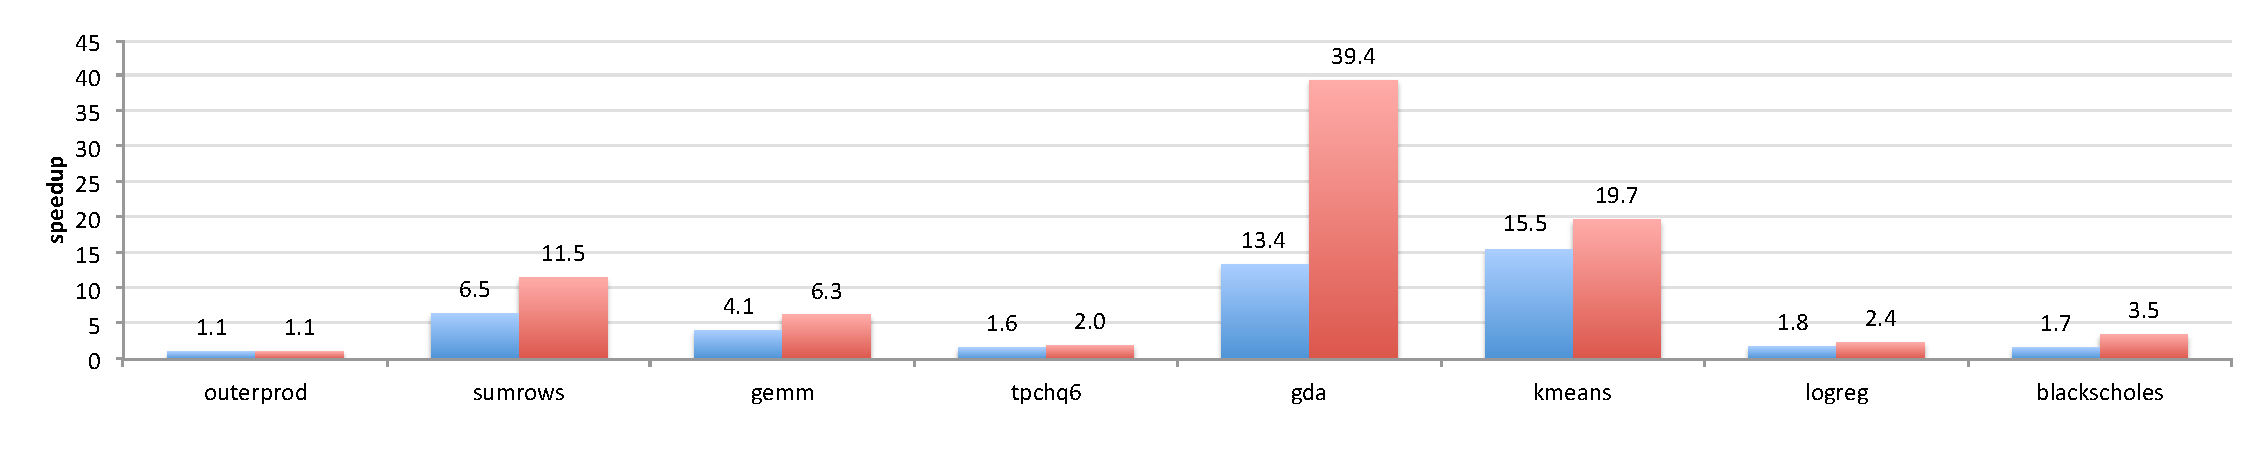
\includegraphics[width=\textwidth]{3-delite/figs/newspeedupbars1.pdf}
\vspace{10pt}
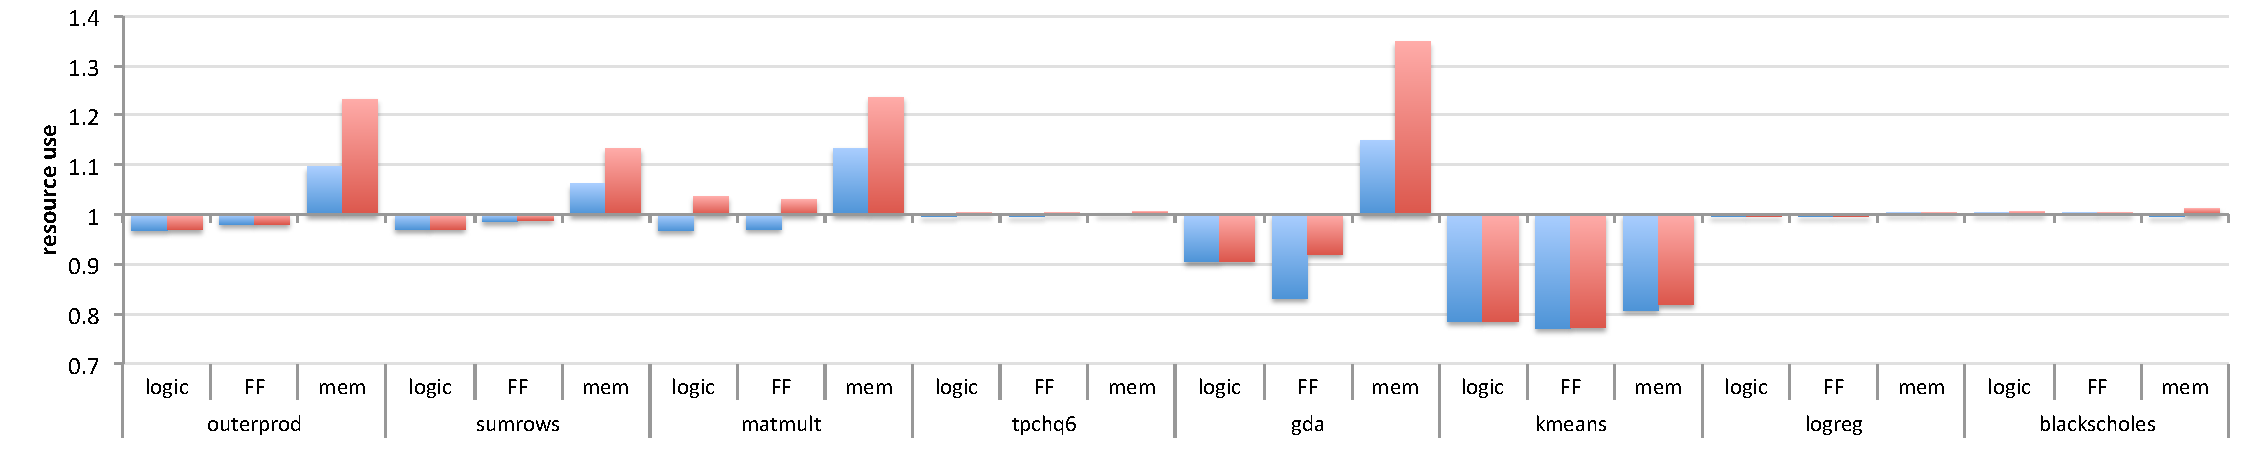
\includegraphics[width=\textwidth]{3-delite/figs/newspeedupbars2.pdf}

{
\fontfamily{phv}\selectfont
\footnotesize
% \raisebox{-0.2em}{\tikz{\path[fill=bar3] (0,0) rectangle (2em,1em);}}
% base design
% \hspace{2em}
\raisebox{-0.2em}{\tikz{\path[fill=bar1] (0,0) rectangle (1em,1em);}}
+tiling
\hspace{2em}
\raisebox{-0.2em}{\tikz{\path[fill=bar2] (0,0) rectangle (1em,1em);}}
+tiling+metapipelining
}

\caption{Speedups and resource usages, relative to respective baseline designs, resulting from tiling and metapipelining.}
\label{fig:speedup-bars}
\end{figure}

\paragraph{Impact of tiling alone}
Figure \ref{fig:speedup-bars} shows the obtained speedups as well as relative on-chip resource utilizations for each of the benchmarks.
As can be seen, most benchmarks in our suite show significant speedup when tiling
transformations are enabled. Benchmarks like \emph{sumrows} and \emph{gemm}
benefit from inherent locality in their memory accesses. For \emph{gemm}, our automatically generated code
achieves a speedup of $4\times$ speedup over the baseline for a marginal increase of about $10\%$ on-chip memory usage.

%Note, the baseline for \emph{gemm} also exploits locality
%by using a tiling where the number of columns in each tile is equal to one DRAM burst. This means that our baseline
%uses tile sizes $1 \times 96 \times 96$.

Benchmarks \emph{outerprod} and \emph{tpchq6} do not
show a significant difference with our tiling transformations over the baseline.
This is because both \emph{outerprod} and
\emph{tpchq6} are both memory-bound benchmarks. \emph{Tpchq6} streams through the input once without reuse, and streaming
data input is already exploited in our baseline design. \emph{Blackscholes} has a similar data access pattern as \emph{tpchq6},
due to which it achieves a speedup similar to that of \emph{tpchq6}. Hence tiling does not provide any additional benefit.
Most of the locality in \emph{logreg} is already captured at burst-level granularity by our baseline. As a result, \emph{logreg}
achieves a modest speedup of $1.8x$ over the baseline due to tiling.
The core compute pipeline in \emph{outerprod} is memory-bound at the stage writing results to DRAM, which cannot be addressed
using tiling. Despite the futility of tiling in terms of performance, tiling \emph{outerprod}
has a noticeable increase in memory utilization as the intermediate result varies as the square of the tile size.

In \emph{kmeans} and \emph{gda}, some
of the input data structures are small enough that they can be held in on-chip memory. This completely
eliminates accesses to off-chip memory, leading to dramatic speedups of $13.4\times$ and $15.5\times$ respectively
with our tiling transformations. \emph{gda} uses more on-chip memory to store intermediate data. On the other hand, the tiled
version \emph{kmeans} utilizes less on-chip memory resources. This is because the baseline for \emph{kmeans} instantiates multiple
load and store units, each of which creates several control structures in order to read and write data from DRAM. Each of these control
structures includes address and data streams, which require several on-chip buffers. By tiling, we require a smaller number of load and
store units.

\paragraph{Impact of metapipelining}
The second speedup bar in Figure~\ref{fig:speedup-bars} shows the benefits of metapipelining. Metapipelines increase throughput
at the expense of additional on-chip memory used for double buffers.
Metapipelining overlaps design compute with data transfer and helps to hide the cost of the slower stage. Benchmarks like
\emph{gemm} and \emph{sumrows} naturally benefit from metapipelining because the memory transfer time is completely overlapped
with the compute, resulting in speedups of $6.3\times$ and $11.5\times$ respectively. Metapipelining also exploits overlap in
streaming benchmarks like \emph{tpchq6} and \emph{blackscholes}, where the input data is fetched and stored simultaneously with the core computation.

The speedup due to metapipelining is largely determined by balancing between stages. Stages with roughly equal number of cycles benefit
the most, as this achieves the most overlap. Unbalanced stages are limited by the slowest stage, thus limiting performance.
We observe this behavior in \emph{outerprod},
where the metapipeline is bottlenecked by the stage writing results back to DRAM. The metapipeline in \emph{logreg} is bottlenecked
at the stage performing dot products of all the points in the input tile with the \emph{theta} vector. As we only parallelize the
innermost parallel pattern in this work, only a single dot product is produced at a time, even though the dot product itself
is executed in parallel across the point dimensions. On the other hand, applications
like \emph{gda}, \emph{kmeans} and \emph{sumrows} greatly benefit from metapipelining. In particular, \emph{gda} naturally
maps to nested metapipelines that are well-balanced. The stage loading the input tile overlaps execution with the stage
computing the output tile and the stage storing the output tile. The stage computing the output tile is also
a metapipeline where the stages perform vector subtraction, vector outer product and accumulation. We parallelize the vector
outer product stage as it is the most compute-heavy part of the algorithm; parallelizing the vector outer product enables
the metapipeline to achieve greater throughput. This yields an overall speedup of $39.4\times$
over the baseline.
